\documentclass[runningheads,a4paper]{llncs}

\usepackage{amssymb}
\setcounter{tocdepth}{3}
\usepackage{graphicx}
\usepackage{url}
\usepackage{amsmath}
\usepackage{listings}
\usepackage[linesnumbered,ruled,vlined]{algorithm2e} 
\usepackage[utf8]{inputenc} % NEW
\usepackage[OT2,T1]{fontenc} % NEW

\newcommand\textcyr[1]{{\fontencoding{OT2}\fontfamily{wncyr}\selectfont #1}}

\newenvironment{itemize2}
       {\begin{itemize}
                \vspace{-0.25em}
                 \setlength{\abovedisplayskip}{0pt}
                 \setlength{\belowdisplayskip}{0pt}
                 \setlength{\itemsep}{4pt}
                 \setlength{\parskip}{0pt}
                 \setlength{\parsep}{0pt}
                 \setlength{\topsep}{0pt}
                 \setlength{\partopsep}{0pt}
         }
         {\vspace{-0.25em}
         \end{itemize}}
}

\newenvironment{enumerate2}
       {\begin{enumerate}
                \vspace{-0.25em}
                 \setlength{\abovedisplayskip}{0pt}
                 \setlength{\belowdisplayskip}{0pt}
                 \setlength{\itemsep}{4pt}
                 \setlength{\parskip}{0pt}
                 \setlength{\parsep}{0pt}
                 \setlength{\topsep}{0pt}
                 \setlength{\partopsep}{0pt}
         }
         {\vspace{-0.25em}
         \end{enumerate}}
}

\urldef{\mailsa}\path|{a.panchenko}@digsolab.com|    
\newcommand{\keywords}[1]{\par\addvspace\baselineskip
\noindent\keywordname\enspace\ignorespaces#1}

\begin{document}

\mainmatter  

\title{Detecting Gender by Full Name: Experiments with the Russian Language}

\titlerunning{Detecting Gender by a Full Name: Experiments with the Russian Language}

\author{Alexander Panchenko\inst{1,2} \and Andrey Teterin\inst{1}  }

%\author{First Name\inst{1} \and Second Author\inst{1} }

\authorrunning{A. Panchenko and A. Teterin}

%\authorrunning{First and Second }

\institute{
Digital Society Laboratory LLC, Moscow, Russia 
%\url{a.teterin@digsolab.com}     
\and
Universit\'{e} catholique de Louvain, Louvain-la-Neuve, Belgium 
\url{alexander.panchenko@uclouvain.be}
}

%\institute{
%Affilation 
%\url{email@email.com}   
%}

\toctitle{ \ldots } 
\tocauthor{ \ldots }
\maketitle


\begin{abstract}

This paper describes a method that detects gender of a person by his/her full name. While some approaches were proposed for English language, little has been done so far for Russian. We fill this gap and present a large-scale experiment on a dataset of 100,000 Russian full names from Facebook. Our method is based on three types of features (word endings, character $n$-grams and dictionary of names) combined within a linear supervised model. Experiments show that the proposed simple and computationally efficient approach yields excellent results achieving accuracy up to 96\%.


\keywords{ gender detection, short text classification.}
\end{abstract}

\section{Introduction}

The Web is full of user-generated content: a plethora of platforms and technologies let a user create comments, posts and other types of textual messages. Most of the time, some information about author of a given text is available. In its simplest form, an author is represented with a \textit{name string}, being either a real name or an alias. While some platforms, such as Facebook and Google+, let the user indicate gender, age and other information, others, such as Twitter or Web forums do not. Furthermore, in most of the platforms, only a name string is required, while other fields, such as gender, can be left unspecified. This is why often only two things can be used to describe a user: her name string and her texts.

However, in many cases it is desirable to know more about an author of a given piece of user-generated content. For instance, in the Internet marketing information about gender and age helps to improve targeting of advertisements~\cite{twitter2012gender}. In cyber security, user profiling can help track down Internet predators and assist in investigations of crimes~\cite{peersman2011predicting}. In information retrieval, sociodemographic  attributes can help customize user search experience and provide more relevant results~\cite{kharitonov2012gender,bi2013inferring}. 

All these factors motivate the need for systems that infer gender, age and other latent sociodemographic attributes of a user. In this paper, we investigate one particular task in this research direction -- \textit{gender detection}. In particular, we focus on gender recognition of Russian full names. The goal of our method is to guess gender of a person by her name. Such a technology can be of use when a true user name is known, but gender was not specified, e.g. for analysis of Twitter users.       

There have been some attempts to propose a method for automatic gender recognition (see Section~\ref{sec:related}). Major limitations of the prior researches are following: (i) most of the studies focus on gender recognition using text written by a person, neglecting full name of a user; (ii) most of the prior works deal with English language, neglecting particularities of other languages, such as Russian. Indeed, most researchers have focused on gender detection by text~\cite{peersman2011predicting,koppel2002automatically,goswami2009stylometric,rangel2013use,nguyen2013old,ciot2013gender,rao2010classifying} with some exceptions, such as~\cite{burger2011discriminating}. Accuracy of the state-of-the-art approaches in this field is about 80-90\%. However, in practical tasks higher accuracy is desirable. We show that one can recognize gender of a person with accuracy higher than 95\% if a full name is available (it is normally the case in social networks and blogs).

Our work fills the gaps mentioned above, as we study gender recognition methods for Russian language based on full name of a person. The main contributions of this paper are as follows. First,  we show that for Russian language, the problem is not very difficult. Even a simplest statistical model yields accuracy of 85\%. Second, we propose a more sophisticated, yet simple and efficient, method that is able to recognize gender of a Russian name with accuracy and precision up to 96\%. 

It is possible that some Russian Internet companies, such as Yandex~\footnote{\url{http://www.yandex.com/}} and Mail.ru~\footnote{\url{http://www.mail.ru/}} already developed technologies similar to ours~\cite{daniel2013research}. However, to the best of our knowledge, we are the first to openly describe details of such technology for the Russian language. A live demo of our method is freely available online~\footnote{ \url{http://research.digsolab.com/gender}}.

\section{Related Work}
\label{sec:related}

Gender of a text author is often known. This makes it easy to build a training corpus of articles, blogs or posts labeled with gender tags.  Provided that the gender detection technology has immediate applications ranging from marketing to cyber-security, no wonder many researchers tried to build supervised models predicting gender by text. 

Koppel et al.~\cite{koppel2002automatically} describe an approach that identifies gender of an author of a written document. In this experiment a genre-labeled subset of the BNC corpus~\footnote{\url{http://www.natcorp.ox.ac.uk/}} was used. The proposed method relies on  combination of lexical and syntactic features and yields accuracy of roughly 80\%. The best performance in this experiment was achieved by a linear model based on function words and parts-of-speech $n$-grams.

Goswami et al.~\cite{goswami2009stylometric} describe a gender detection experiment with 9,660 gender-labeled blog posts from the \url{blogger.com} platform. Features used in this experiment include slang words statistics, sentence length and other stylometric parameters. The proposed model yields accuracy of 89.3\%.

Mukherjee and Liu~\cite{mukherjee2010improving} propose two novel approaches to gender classification. The first is based on variable length POS sequences, while the second relies on automatic feature selection. The authors report increase in accuracy due to these features from 79.6\% to 88.6\% on a collection of 3,100 gender-labeled blogs from the \url{blogger.com}.

Peersman et al.~\cite{peersman2011predicting} describe a method for short text classification by gender. The authors deal with a gender-balanced corpus of messages coming from the Dutch social network \textit{Netlog}. The proposed technique relies on an SVM classifier~\cite{vapnik} with features based on word/character unigrams, bigrams and trigrams. The best accuracy score of 88,8\% in this experiment was achieved with a model based on 50,000 most informative word unigrams selected with $\chi^2$ test.

Daniel and Zelenkov~\cite{daniel2013research} performed a statistical analysis of the spoken sub-corpus of the Russian National Corpus~\footnote{\url{http://www.ruscorpora.ru/en/}}. It appeared that in public communication there is a statistically significant difference between the speech of men and women (men talk more), while the same difference is absent in private communication. The article also mentions a gender recognition system for written texts with accuracy ``about 90\%'' trained on the same corpus. 

It is worth mentioning that age and gender prediction have much in common. First, often researchers tackle two these problems in the same study~\cite{rangel2013use,peersman2011predicting,goswami2009stylometric}. Second, the state-of-the-art techniques for age and gender prediction are fairly similar. In their simplest form these methods are based on supervised linear models trained on character and/or lexical unigrams. Nguyen et al.~\cite{nguyen2013old} also points out an interaction between age and gender variables. Furthermore, the authors study impact of gender on quality of age prediction. For instance, it was found that age prediction works better for females.   

Ciot et al.~\cite{ciot2013gender} were among the first to present an experiment on non-English data. The authors tackled the gender recognition problem of French, Japanese, Indonesian and Turkish texts.  This study revealed that (i) the methods working well in English yield good results as well for French, Turkish and Indonesian; (ii) baseline methods provide poor results for Japanese; (iii) language-specific features can boost accuracy of the baseline approach. 

The work of Burger et al.~\cite{burger2011discriminating}  is arguably the one most similar to our research. The authors proposed a model based on features extracted both from texts written by a person and his full name. The study is based on a dataset of 184 thousand Twitter users speaking more than 13 languages. However, Russian-speaking users were not studied in this experiment. Similarly to other researchers, Burger et al. used supervised models trained on character and word $n$-grams. Their model based on full names achieved an accuracy of 89\%, while the model based on all text fields of Twitter profile provided an accuracy of 92\%.  

Thus, recently gender detection technology received a significant attention in the literature. Some further related experiments include Rao et al.~\cite{rao2010classifying}, Rangel and Rosso~\cite{rangel2013use}, Al Zamal et al.\cite{al2012homophily} and Lui et al.~\cite{liu2012using}.
  

\section{Dataset}

We performed our experiments on a dataset of 100,000 names of Facebook users with publicly available profiles. Each such \textit{name string} contains first and last name of a user or whatever information the user inserted into this field instead. Each name string has a gender label: \textit{male} or \textit{female}. We did not consider users with unknown gender. The dataset was collected with the Facebook API~\footnote{\url{https://developers.facebook.com/tools/explorer}} from publicly available profiles of Russian-speaking users. The dataset contains both names written in Cyrillic and Latin alphabets, e.g. ``Alexander Ivanov'' and its Cyrillic equivalent \textcyr{``Александр Иванов''}. 

Fig.~\ref{fig:matrix} lists the most frequent names and surnames in the dataset. Here and below we present transliterated versions of Cyrillic characters. In our experiment, we considered the first token of a name string as a given name and the second one as a surname. It is clear from the table that in Russian language: (i) information about gender is encoded in the endings; (ii) there is a gender agreement. For instance, ``Alexandr Ivanov'' is a man's name, ``Alexandr\textbf{a} Ivanov\textbf{a}'' is a woman's name, and ``Alexandr Ivanov\textbf{a}'' is an ungrammatical name.   

While our dataset represents a significant number of common Russian names, some rare names are under-represented. For instance, the female name ``Oksana Kim'', is a relatively rare, but a perfectly valid female name. Yet, it is not present in our dataset (see Fig.~\ref{fig:matrix}). However, there are 745 people with the first name ``Oksana'' and 70 persons with the last name ``Kim''.  


\begin{figure}
\centering
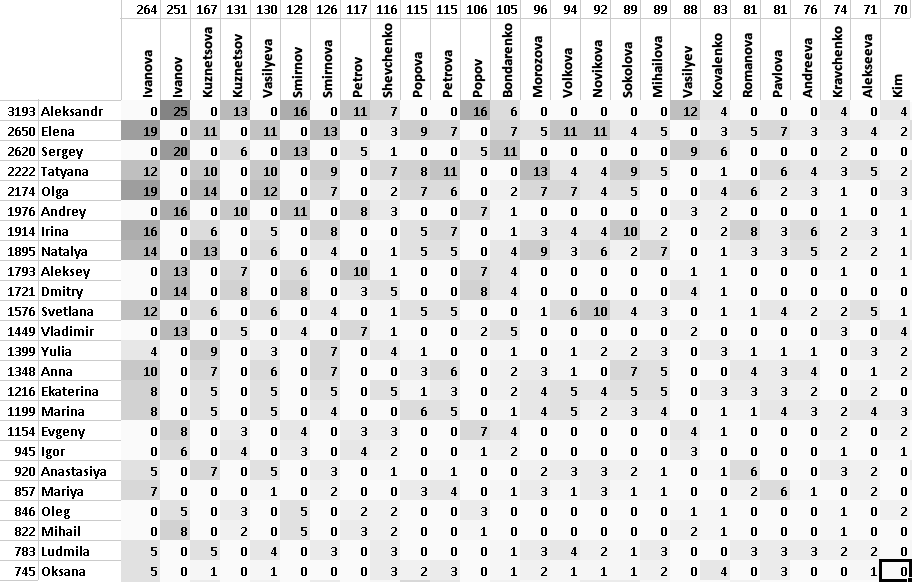
\includegraphics[width=1.0\textwidth]{figures/matrix3} 
\caption{ Name-surname co-occurrences: rows and columns are sorted by frequency. }
\label{fig:matrix}
\end{figure}

In order to assess difficulty of the gender recognition task, we analyzed endings of first and last names in a sample of 10,000 objects. In this context, an \textit{ending} is a substring composed of last two characters of a first/last name. According to this experiment, 72\% of first names and 68\% of surnames have typical male/female ending. Here a \textit{typical male/female ending} is an ending that splits males from females with an error less than 5\% (see Table~\ref{tab:endings}). It appears that gender of more than 50\% given names from our sample can be robustly detected with 8 endings. Furthermore, gender of more than 50\% second names can be recognized with only 5 endings (see Table~\ref{tab:endings}). These observations suggest that a simple symbolic ending-based method cannot robustly classify about 30\% of names. This motivates the need for a more sophisticated statistical approach. 


\begin{table}[h]

\footnotesize

\begin{center}
\begin{tabular}{|l|ll|l|l|l|l|}
\hline
\bf Type & \bf Ending & & \bf Gender & \bf Error, \% &  \bf Example \\ \hline \hline

first name & na & (\textcyr{на}) & female & 0.27 & Ekateri\textbf{na} \\
first name & iya & (\textcyr{ия}) & female & 0.32 & Anastas\textbf{iya} \\
first name & ei & (\textcyr{ей}) &  male & 0.16 & Serg\textbf{ei} \\
first name & dr & (\textcyr{др}) & male & 0.00 & Alexan\textbf{dr} \\
first name & ga & (\textcyr{га}) & male & 4.94 & Sere\textbf{ga} \\
first name & an  & (\textcyr{ан}) & male & 4.99 & Iv\textbf{an} \\
first name & la & (\textcyr{ла}) & female & 4.23 & Luidmi\textbf{la} \\
first name & ii & (\textcyr{ий}) & male & 0.34 & Yur\textbf{ii} \\
second name & va & (\textcyr{ва})  & female & 0.28 & Morozo\textbf{va} \\
second name & ov & (\textcyr{ов})  & male & 0.21 & Objedk\textbf{ov} \\
second name & na & (\textcyr{на})  & female & 2.22 & Matyushi\textbf{na} \\
second name & ev & (\textcyr{ев}) & male & 0.44 & Serge\textbf{ev} \\
second name & in & (\textcyr{ин}) & male & 1.94 & Teter\textbf{in} \\
 
\hline
\end{tabular}
\end{center}
\caption{ Most discriminative and frequent two character endings of Russian names.  }
\label{tab:endings}
\end{table}

\section{Gender Detection Method}

The gender detection method takes as input a string representing a name of a person and outputs a gender (male or female). A name string is usually extracted from a user profile. Thus, we tackle the problem as a binary classification task. A label with unknown gender can be obtained by means of the reject option~\cite[p.42]{bishop2006pattern}. Below we describe features and the model used in our gender recognition approach. This section is concluded with a description of a simple rule-based baseline.

\subsection{Features}

In our experiments, we used three types of features based respectively on endings, character $n$-grams and a dictionary of male/female names and surnames. 

\subsubsection{Word endings}

As we already mentioned above, Russian language, unlike English, has a gender agreement. Thus, the same name or surname often has different endings for a male and a female:
\begin{itemize2}
\item males: Alexander Yaroskavski, Oleg Arbuzov
\item females: Alexandr\textbf{a} Yaroskavska\textbf{ya}, Nayali\textbf{ya} Arbuzov\textbf{a}
\end{itemize2}
Thus, some Russian surnames are transliterated differently for males and females (see above). However, other surnames are spelled in the same way for both genders, e.g. ``Sidorenko'', ``Moroz'' or ``Bondar''.   

The two most common one-character endings of female names/surnames are ``a'' and ``ya'' (``\textcyr{я}'' in Cyrillic). We use four features that indicate on female gender in Russian language: (1) first name ends with ``\textcyr{а}'', (2) first name ends with ``\textcyr{я}'', (3) last name ends with ``\textcyr{а}'', (4) last name ends with ``\textcyr{я}''.

\subsubsection{Character $n$-grams}

These features rely on character unigrams, bigrams or trigrams extracted from the name strings. We represent a name with $k$ its most frequent $n$-grams. The extraction is done with help of the NLTK module~\cite{bird2006nltk}. 

Most frequent trigrams are listed below (here ``\_'' denotes a beginning or an end of a name string): a\_\_, va\_, v\_\_, {na }, ova, \_\_A, ov\_, ina, kov, nov, \_Al, n\_\_, a\_\_, o\_\_, \_\_V, ndr, Ale, {iya }, {ei }, {lek}, {eks}, {ko\_}, {nko}, {rin}, {\_An}, {enk}, {\_\_C}, {na\_}, ``{ii }'', {\_\_E}, {eva}, {\_\_N}, {\_\_M}, {san}, {ksa}, {\_\_I} , {ev\_} , {in\_}, {and}, {len}, {\_\_O}, {va\_}, {rov}, {\_Na}. Note that the most frequent trigrams are not necessarily the most discriminative, e.g. ``ko\_'' is a common surname ending for both males and females.


\subsubsection{Dictionaries of first and last names}

This type of features is based on dictionaries of first and last names. Each entry of a dictionary contains a first/last name and a probability that it belongs to the male gender:
$$
P(c=male|w) = \frac{n_{male}^w }{\sum_{c \in \{male, female\}} n_{c}^w}, 
$$
where $n_{male}^w$ is a number of male profiles with the first/last name $w$ in the dictionary. We use two dictionary-based features: (1) probability that first name is of male gender $P(c=male|firstname)$, (2) probability that the last name is of male gender $P(c=male|lastname)$. 

We used 90,000 name strings to build the two dictionaries. The training set used in our experiments does not contain any of these 90,000 samples. In order to remove noisy entries, we deleted all names and surnames that occurred only once. The full dictionary of first names contained 3,427 entries, while the dictionary of last names contained 11,411 entries. We used several versions of these full dictionaries in our study. Each version included top $\gamma$\% most frequent given names and surnames.    

\subsection{Model}

In all our experiments we used L2-regularized \textit{Logistic Regression} model~\cite{agresti2002categorical} as it generally yields reasonable results for the NLP-related problems~\cite{panchenko2013towards}.
% For instance, prior experiments with a different short text classification problem has shown a little variation between various linear models. Therefore, in this paper we try various features, keeping the same model in each run. 
Let $y_i \in \{-1,+1\}$ be a gender label and $\mathbf{x} = (x_1,\ldots,x_n)$ be a set of features  representing a name string. The logistic regression combines features in a linear combination with weights $\mathbf{w}$. This weight vector is obtained by minimizing the following unconstrained optimization problem~\cite{fan2008liblinear}:  
$$
\min_{\mathbf{w}} \sum_i log (1 + e^{-y_i\mathbf{w}^T \mathbf{x}_i}) + \frac{1}{C} || \mathbf{w} ||_2
$$
We use the \texttt{scikit-learn} module in this experiment~\footnote{\url{http://scikit-learn.org/}}. This implementation relies on the Dual Coordinate Descent Method for training of the model~\cite{yu2011dual}. Default meta-parameters of the model were used. The model uses nearly no regularization -- the inverse of the regularization strength $C$ was set to 100,000. Optimization of the meta-parameters, such as $C$,  or using more sophisticated models, such as SVM~\cite{vapnik} can lead to significant improvements in results. However, in this paper we focus on a comparison of different features used withing the framework of one model. 

The model $\mathbf{w}$ can be applied to perform classification of a name string represented with a feature vector $\mathbf{x}$ as follows:
$$
P(y=1|\mathbf{x}) = \frac{1}{1 + e^{-\mathbf{w}^T \mathbf{x}}  }.
$$


\subsection{Rule-based Baseline}

There exist several available spelling dictionaries of Russian male and female first names, such as: 

\begin{itemize2}

\item a reference dictionary of personal names~\footnote{\url{http://imena-list.ru/}};

\item a dictionary of personal names of Russian language by F. L. Ageenko~\footnote{\url{http://www.gramota.ru/slovari/info/ag/}};

\item category ``Names'' of Russian Wiktionary~\footnote{\url{http://ru.wiktionary.org/wiki/}\textcyr{Категория:Имена}};

\item Russian spelling dictionary of Wikisource~\footnote{\url{http://ru.wikisource.org/wiki/}\textcyr{Орфографический\_словарь\_русского\_языка}}.

\end{itemize2}

These dictionaries can be used to classify full names by gender. We compiled a dictionary of 1,428 Russian first names labeled with gender from Wiktionary and Wikisource~\footnote{Available at \url{http://panchenko.me/gender/wiki-gender-dict.csv}}. This dictionary has no names assigned to both male and female categories.The dictionary was used to implement a rule-based baseline that works as follows. First, an   input name string is transformed into a set of tokens $t$. Let $d_f$ be a set of female first names and $d_m$ be a set of male first names. Second, gender $c$ is assigned to a full name with the following rule:

$$
c = \begin{cases}
    male, & \mbox{if } (t \cap d_m \neq \emptyset) \mbox{ and } (t \cap d_f = \emptyset), \\
    female, & \mbox{if } (t \cap d_m = \emptyset) \mbox{ and } (t \cap d_f \neq \emptyset), \\
    unknown, & \mbox{else}.
    \end{cases}
$$

Thus, a person with a female first name will be considered as a female, while a person with an unknown first name will have no gender label. 


\section{Results and Discussion}

In this section, we present results of the experiments with the gender classification approaches described above. We start with the results of the rule-based baseline. Next, we proceed to statistical models based on one type of features: endings, character trigrams and dictionary. Finally, we present results of the statistical models that rely on several kinds of features at the same time. 

Table~\ref{tab:results} presents main results of our experiments in terms of the standard performance metrics calculated on a sample of 10,000 name strings. Among these 10,000 names we found 127 (1.27\%) duplicate names. Fig.~\ref{fig:curve} illustrates how size of the training set affects accuracy. 

\begin{table}[h]

\footnotesize

\begin{center}
\begin{tabular}{|l|l|l|l|l|}
\hline
\bf Model & \bf Accuracy & \bf Precision & \bf Recall & \bf F-measure \\ \hline \hline

\textit{rule-based baseline} &  0,638 & \bf 0,995 & 0,633 & 0,774 \\   

\textit{endings} & 0,850 $\pm$ 0,002 & 0,921 $\pm$ 0,003 & 0,784 $\pm$ 0,004 & 0,847 $\pm$ 0,002 \\

\textit{3-grams} & 0,944 $\pm$ 0,003 & 0,948 $\pm$ 0,003 & 0,946 $\pm$ 0,003 & 0,947 $\pm$ 0,003 \\

\textit{dicts} & 0,956 $\pm$ 0,002 & \bf 0,992 $\pm$ 0,001 & 0,925 $\pm$ 0,003 & 0,957 $\pm$ 0,002 \\ 

\textit{endings+3-grams} & 0,946 $\pm$ 0,003 & 0,950 $\pm$ 0,002 & 0,947 $\pm$ 0,004 & 0,949 $\pm$ 0,003 \\

\textit{3-grams+dicts} & 0,956 $\pm$ 0,003 & 0,960 $\pm$ 0,003 &  0,957 $\pm$ 0,004 &  0,959 $\pm$ 0,003 \\ 
 
\textit{endings+3-grams+dicts} & \bf 0,957 $\pm$ 0,003 & 0,961 $\pm$ 0,003 & \bf 0,959 $\pm$ 0,004 & \bf 0,960 $\pm$ 0,002  \\

\hline
\end{tabular}
\end{center}
\caption{ Results of the experiments on the training set of 10,000 names (10-fold cross-validation). Here \textit{endings} -- 4  Russian female endings, \textit{trigrams} -- 1000 most frequent 3-grams, \textit{dictionary} -- name/surname dictionary with $\gamma=80\%$ top entries. This table presents precision, recall and F-measure of the female class. }
\label{tab:results}
\end{table}

\subsection{Rule-based Baseline} As one can see, the rule-based classifier is very precise. It achieves precision of 0.995. However recall of this method is only 0.663. This is due to a large number of unclassified examples: the dictionary used by this classifier does not list many first names common on Facebook. 

\subsection{Word endings} As to the statistical classifiers, even the simplest model that relies on two female endings ``\textcyr{а}'' and ``ya'' (``\textcyr{я}'') yields reasonable results, achieving accuracy up to 0.850.  However, while precision of such a naive model is relatively high (0.921), its recall is only 0.784. Therefore, a significant fraction of female names do not follow simple ending-based rules. Naturally, performance of the ending-based model improves a little as training set grows (see Fig.~\ref{fig:curve}). A hundred of examples is sufficient for training.  

\subsection{Character $n$-grams}
In these experiments we focus on trigrams, as according to our results they worked better than bigrams and unigrams. Table~\ref{tab:results} and Fig.~\ref{fig:curve} present performance of the models based on 1,000 most frequent trigrams. Character trigrams  significantly outperform word endings if a training set is larger than 30 samples. Furthermore, unlike the ending-based model, the trigram-based model  improves as the training set grows reaching accuracy of 0.944 on a dataset of 10,000 samples.

\begin{figure}
	\centering
	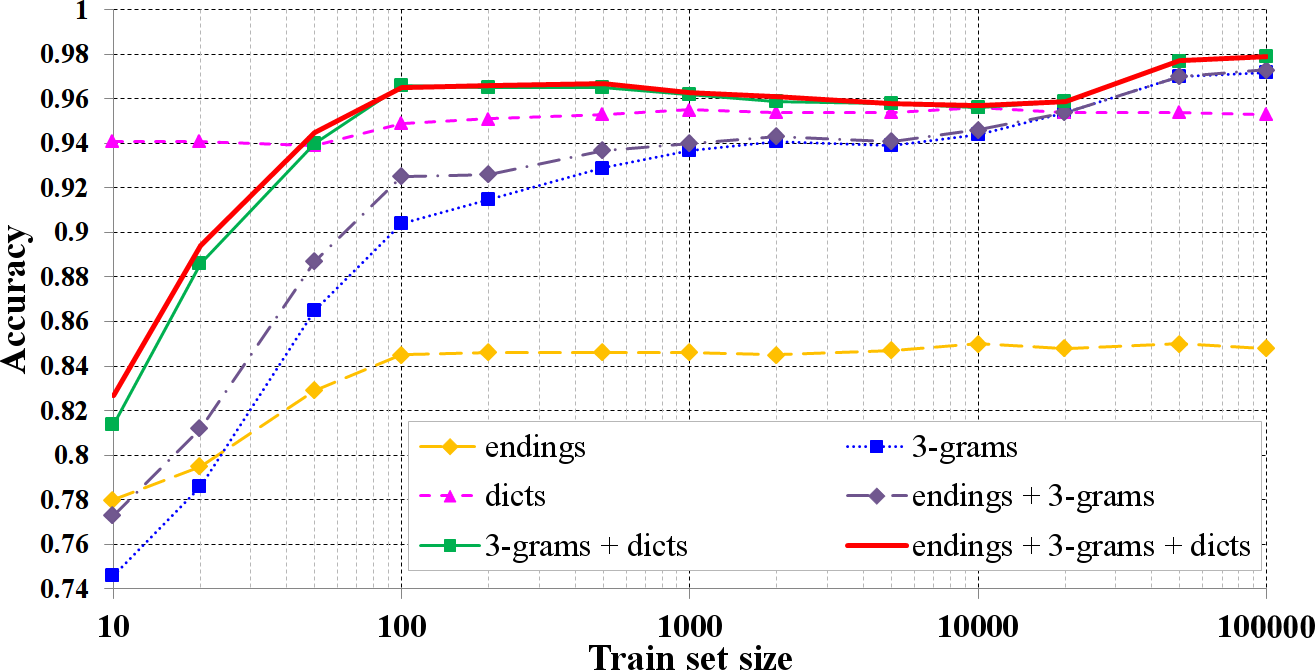
\includegraphics[width=1.0\textwidth]{figures/lc-all} 
	\caption{ Learning curves of single and combined models. Accuracy was estimated on separate sample of 10,000 names.  }
	\label{fig:curve}
\end{figure}

Fig.~\ref{fig:ngrams} plots accuracy of the  \textit{3-grams} model function of the number of most frequent trigrams used. In our further experiments (the combined models e.g.\textit{3-grams+dicts}) we used a model based on top 1000 trigrams as a good trade-off between computational complexity and accuracy. 

\begin{figure}
\centering
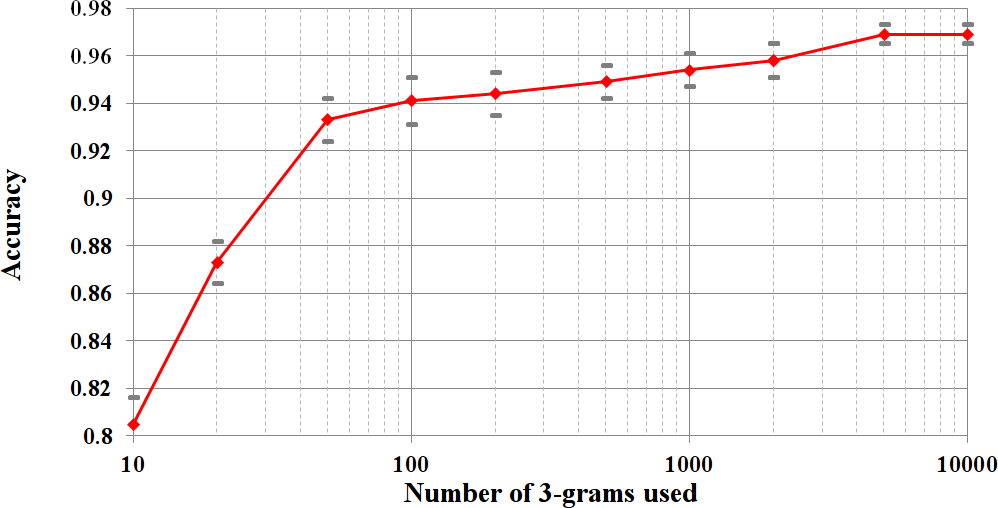
\includegraphics[width=1.0\textwidth]{figures/ngrams} 
\caption{ Accuracy of the model \textit{3-grams} function of the number of features used $k$. }
\label{fig:ngrams}
\end{figure}

\subsection{Dictionary of first and last names} The model \textit{dicts} that relies on a dictionaries of given names and surnames yields very competitive results (accuracy up to 0.956). Furthermore, this model provides the best precision among all statistical models (0.992). However, its recall is significantly lower than that of trigrams and combined models. As one may expect, only several dozens of training examples are enough to train this model (see Fig.~\ref{fig:curve}). Further increase of the training set naturally does not improve accuracy as (i) it has only two features; (ii) the dictionaries are extracted from an independent part of data, not from the training set. 

Fig.~\ref{fig:dict} plots accuracy of the \textit{dicts} model function of the dictionary size $\gamma$. The maximal accuracy is achieved if the full dictionary is used ($\gamma = 100\%$). However, in our experiments we used $\gamma = 80\%$ of the dictionaries (2,741 first names and 9,128 last names) as the difference between the two respective dictionary-based models is minimal. In fact, even if one would use only $\gamma = 60\%$ of the dictionaries (2,056 first names and 6,846 last names) one will get nearly the same results.   


\begin{figure}
\centering
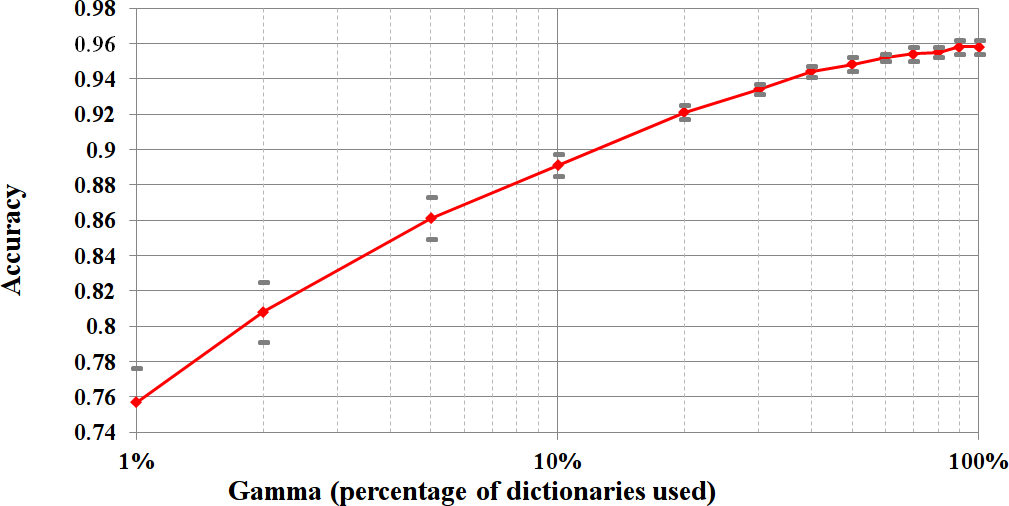
\includegraphics[width=1.0\textwidth]{figures/dict} 
\caption{ Accuracy of the \textit{dicts} model function of the fraction of dictionaries used $\gamma$. }
\label{fig:dict}
\end{figure}

\subsection{Combined Models} We experimented with three combined models: \textit{endings+3-grams}, \textit{3-grams+dicts} and \textit{endings+3-grams+dicts}. Combination of trigrams with word endings yields nearly the same performance as the model based on trigrams only. Indeed, the two female endings ``\textcyr{а}'' and ``ya'' (``\textcyr{я}'') are present among frequent trigrams, such as ``\textcyr{а\_\_}'', ``{va\_}'', ``{na\_}'', ``{ya\_\_}'', ``{aya\_}'', or ``{iya\_}''.  

On the other hand, the model that relies on both dictionary and trigrams outperforms both trigram- and dictionary-based models, reaching accuracy of 0.956 due to increase in recall. However, precision of this combined model is significantly lower than that of the single dictionary-based model (0.960 versus 0.992). This is so as an $n$-gram model can capture noisy sequences or estimate poorly weights of some $n$-grams due to sparsity of the training data. 

Finally, the model \textit{endings+3-grams+dicts}  that makes use of all three types of features shows slightly higher performance than \textit{3-grams+dicts}.  However, this difference is not statistically significant. As we already discussed above, trigrams model well word endings. Table~\ref{tab:errors} lists some errors produced by our best model \textit{endings+3-grams+dicts} on test and train sets. Train set error is very small (about 0.3\%), while test set error is bigger (about 4\%). There are several types of errors: 

\begin{itemize2}
\item Inconsistent annotation, such as ``Anna Kryukova (male)'' or ``Boris Krolchansky (female)''. 

\item Name string is neither male nor female, but rather a name of a group, e.g. ``Wikom Tools'', ``Kazakh University of Humanities'' or ``Privat Bank''.

\item Name string represents a foreign name, e.g. ``Abdulloh Ibn Abdulloh'', ``Brooke Alisson'', ``Ulpetay Niyetbay'' or ``Yola Dolson''. Our model was not trained to deal with such names. 

\item Meaningless or partially anonymized names names, e.g. ``Crazzy Ma'', ``Un Petit Diable'', ``Vv Tt'', ``Vio La Tor'' or ``Muu Muu''. Additional information is required to derive gender of such users.

\item People with rare names or surnames, e.g. ``Guldjan Reyzova'',  ``Yagun Zumpelich'' or ``Akob Saakan''. These are people with common names and surnames in other countries, such as Georgia, Kazakhstan, Azerbaijan or Tajikistan. In our dataset, people from these countries are under-represented. 

\item Full names that can denote both males and females, e.g. ``Jenya Chekulenko'', ``Jenya Sergienko'', ``Sasha Sidorenko'' or ``Sasha Radchenko''. Additional information is required to infer gender of such people.

\item Misclassifications of common names, e.g. ``Ilya Nasorshin'', ``Oleg Dubovik'' or ``Elena Antropova''. 


\end{itemize2}


\begin{table}[h]

\footnotesize

\begin{center}
\begin{tabular}{|l|ll|ll|}
\hline
 &  \bf Train Set Errors &  & \bf Test Set Errors & \\ \hline 

 &  \bf name & \bf true class & \bf name & \bf true class \\ \hline \hline

1 & Lea Shraiber  & female & Ilya Nadorshin & male \\  
2 & Profanum Vulgus  & female & Rustem Saledinov & male \\  
3 & Anna Kryukova & male & Erkin Bahlamet & male \\  
4 & Gin Amaya & male & Gocha Lapachi & male \\  
5 & Gertrud Gallet  & female & Muttaqiyyah Abdulvahhab & female \\  
6 & Dolores Laughter & female & Yola Dolson & female \\  
7 & Di Nolik  & male & Heiran Gasanova & female \\  
8 & Jūlija Hotiņeca  & female & Hadji Murad & male \\  
9 & Gic Globmedic  & female & Jenya Chekulenko & female \\  
10 & Ulpetay Niyetbay  & female & Tury.Ru Domodedovskaya Metro Office & male \\  
11 & Olga Shoff  & male & Elmira Nabizade & female \\  
12 & Phil Golosoun  & male & Niko Liparteliani & male \\  
13 & Tsitsino Shurgaya & female & Oleg Grin' & male \\  
14 & Anna Grobov  & female & Santi Zarovneva & female \\  
15 & Linguini Incident & female & Misha Badali & male \\  
16 & Toma Oganesyan & female & Che Serega & male \\  
17 & Swon Swetik & female & Petr Kiyashko & male \\  
18 & Adel Simon & female & Sandugash Botabaeva & female \\  
19 & Ant Kam-  & male & Jenya Sergienko & female \\  
20 & Xristi Xitrozver  & female & Abdulloh Ibn Abdulloh & female \\  
21 & Anii Reznookova  & female & Naikaita Laitvainenko & male \\  
22 & Aurelia Grishko & male & Fil Kalnitskiy & male \\  
23 & Alex Bu  & female & Helen Hovel' & female \\  
24 & Karen Karine & female & Valery Kotelnikov & male \\  
25 & Russian Spain & female & Max Od & male \\  
26 & Lucy Walter & male & Jean Kvartshelia & male \\  
27 & Aysah Ahmed & female & Adjedo Trupachuli & female \\  
28 & Kiti Iz  & female & Ainur Serikova & female \\  
29 & Cutejilian Juka  & female & Privat Bank & female \\  
30 & Azer Dunja  & male & No Limit & female \\  

\hline
\end{tabular}
\end{center}
\caption{ Examples of train and test set errors of the model \textit{endings+3-grams+dicts}. Here Cyrillic characters were transliterated into English in the standard way. }
\label{tab:errors}
\end{table}


 

\section{Conclusion}

We presented several simple and computationally efficient models for gender detection by a full name of a person. The methods yields excellent results on a dataset Russian-speaking Facebook users, achieving accuracy up to 96\%. In our further research, we plan to complement the developed approach by a gender detection method based on texts written by a person, as a full name is not always available or can give no clue about gender. For instance, the name ``Sasha Sidorenko'' can refer to both a male and a female. 

\section*{Acknowledgements}

This research was supported by Digital Society Laboratory LLC. We thank Kirill Shileev, Segei Objedkov and three anonymous reviewers for their helpful comments that significantly improved quality of this paper.

\bibliographystyle{splncs}
\bibliography{biblio2}

\end{document}
